\documentclass{standalone}
\usepackage{tikz}
\usepackage{graphicx}
\usetikzlibrary{positioning}
\usetikzlibrary{calc}
\def\mainpath{../../}
\def\tikzpath{./}
\def\studypath{/home/lukas/Desktop/SA_Thesis/studies}

\usepackage{import}

\usepackage[outline]{contour}

\usepackage{pgfplots}
\usepackage{pgfplotstable}



%colors for text highlighting
\definecolor{hlcolor_blue}{RGB}{126,215,255}
\definecolor{hlcolor_green}{RGB}{126,255,175}
\definecolor{hlcolor_orange}{RGB}{246,194,115}
\definecolor{hlcolor_yellow}{RGB}{255,243,113}
\definecolor{hlcolor_purple}{RGB}{215,163,232}

%tikz color list
\definecolor{list1_1}{RGB}{0,101,189}
\definecolor{list1_2}{RGB}{156,157,159}
\definecolor{list1_3}{RGB}{162,173,0}
\definecolor{list1_4}{RGB}{227,114,34} 
\definecolor{list1_5}{RGB}{152,198,234}


%\definecolor{list1_1}{RGB}{246,81,29}
%\definecolor{list1_2}{RGB}{255,180,0}
%\definecolor{list1_3}{RGB}{0,166,237}
%\definecolor{list1_4}{RGB}{127,184,0}
%\definecolor{list1_5}{RGB}{13,44,84}


\pgfplotscreateplotcyclelist{markerlist}{
list1_1, thick, solid, mark=*\\%
list1_2, thick, solid, mark=asterisk\\%
list1_3, thick, solid, mark=diamond*\\%
list1_4, thick, solid, mark=triangle\\%
list1_5, thick, solid, mark=square\\%
}

\pgfplotscreateplotcyclelist{linelist}{
list1_1, solid\\%
list1_2, solid\\%
list1_3, solid\\%
list1_4, solid\\%
list1_5, solid\\%
}

\definecolor{lightgrey}{RGB}{200,200,200}
\definecolor{nassitextcolor}{RGB}{0,0,200}
\begin{document}

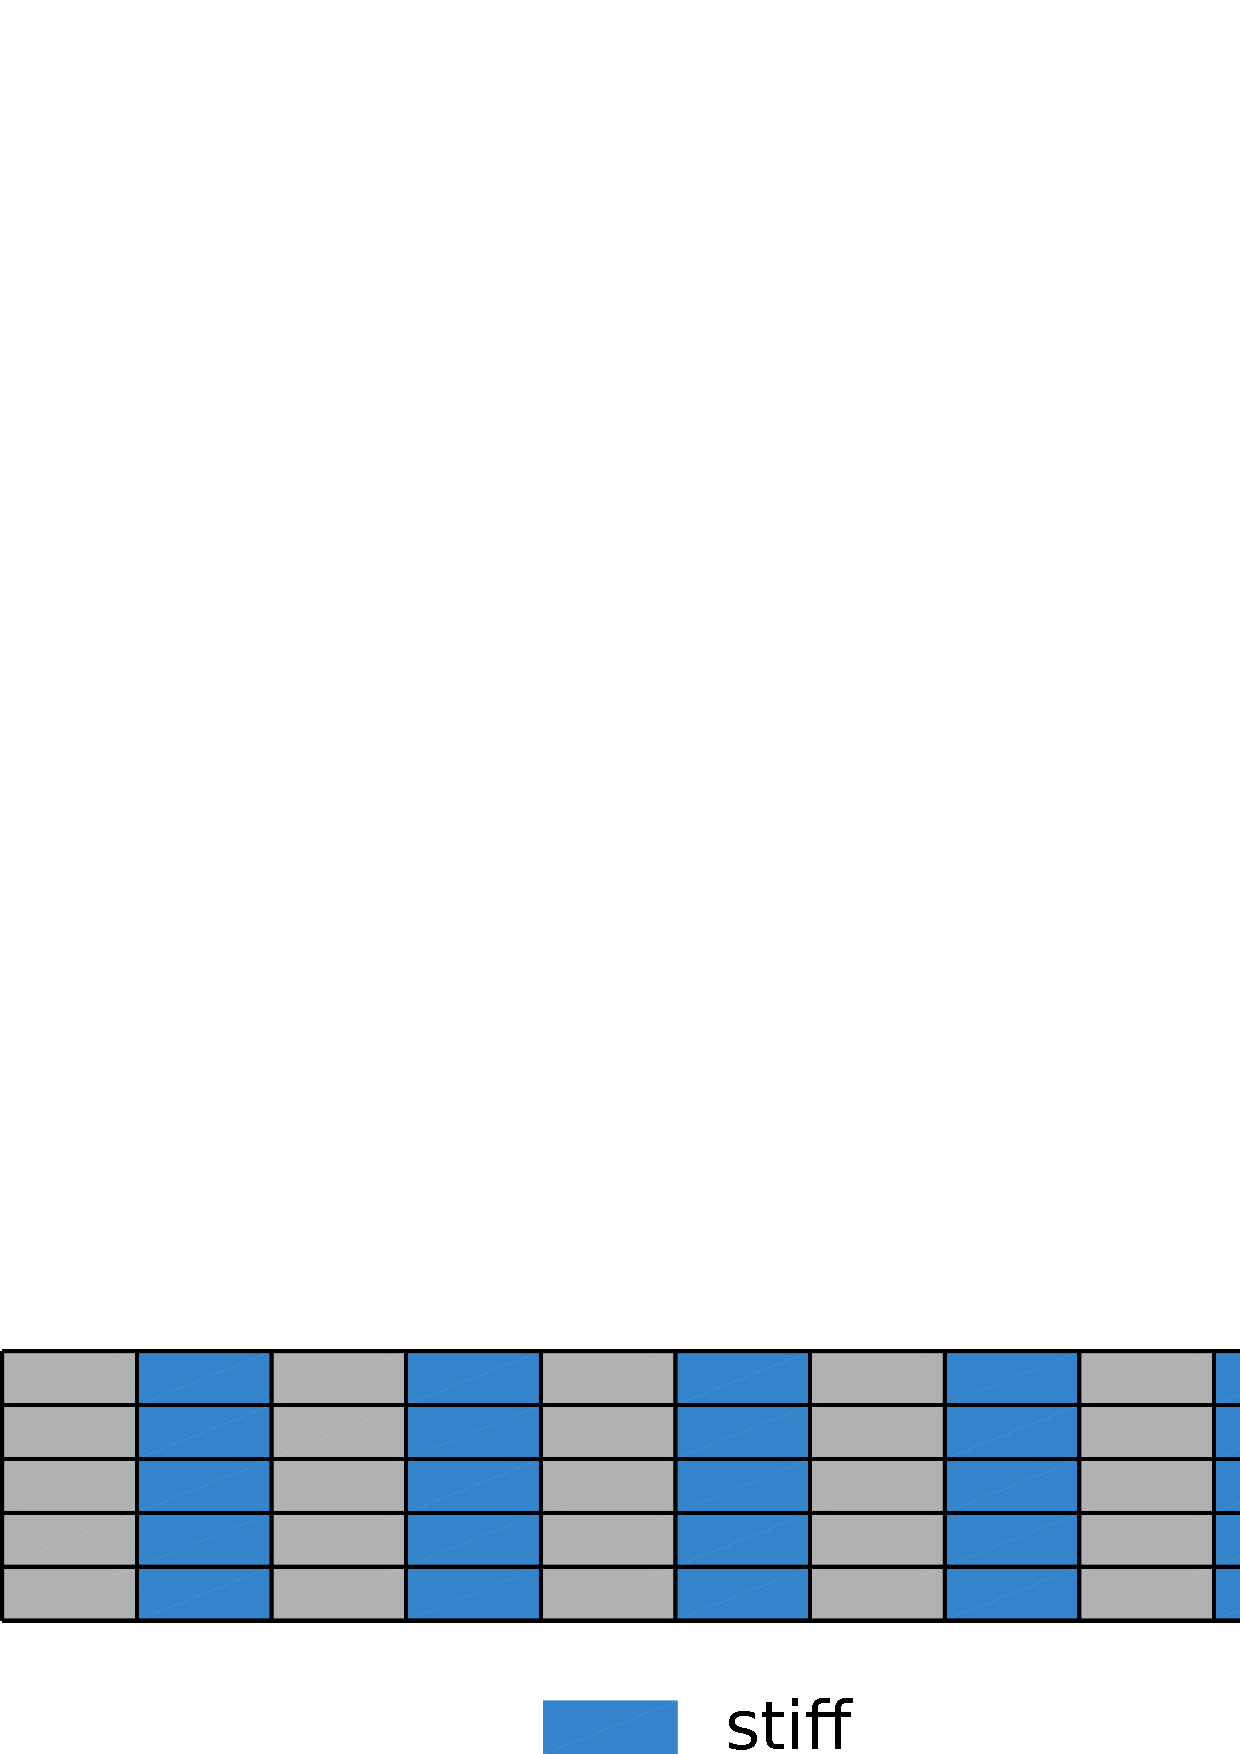
\includegraphics[width=.7\textwidth]{\studypath/2016-08-22_HeterogenityType/setup/materials_vertical.pdf}};


\begin{tikzpicture}
\def\ydist{-2.1}



\node[inner sep=0pt] (russell) at (0,0)
    {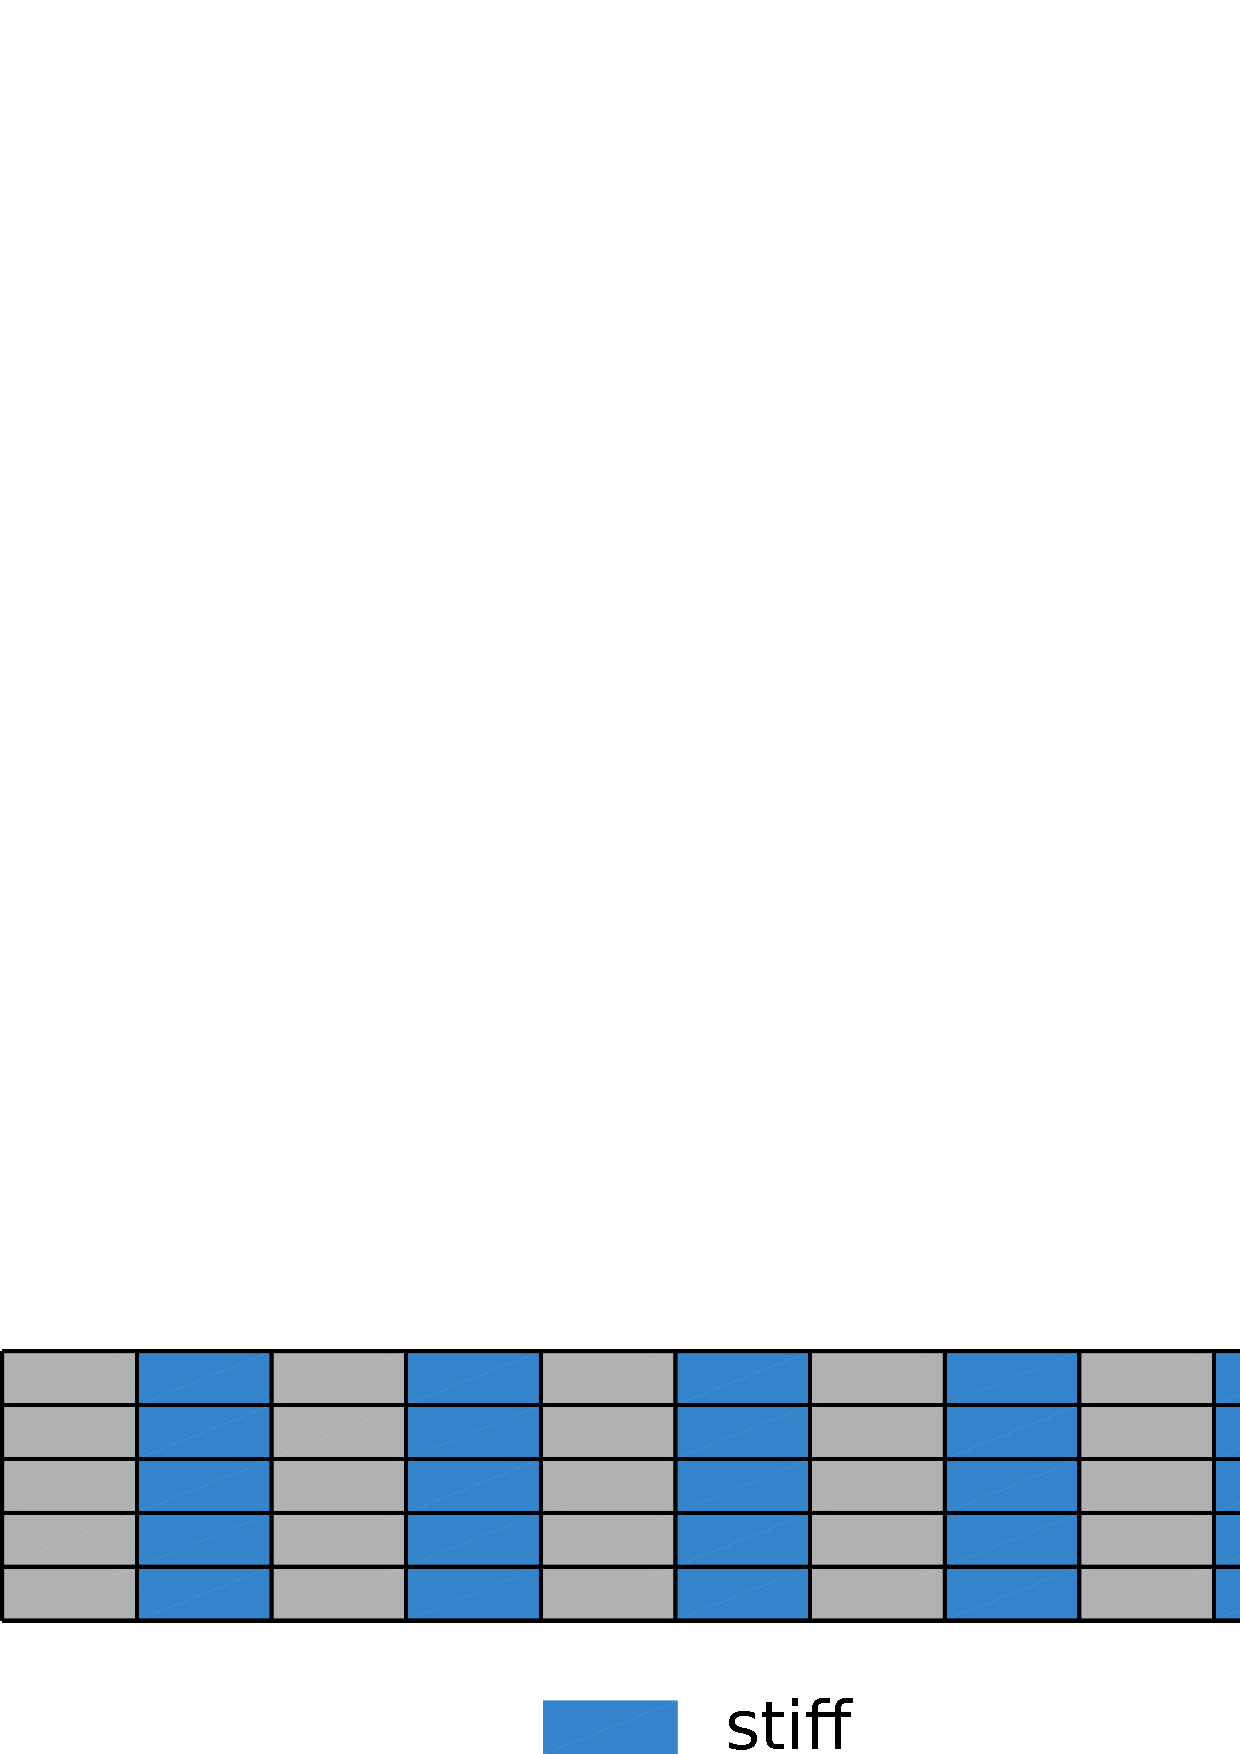
\includegraphics[width=.7\textwidth]{\studypath/2016-08-22_HeterogenityType/setup/materials_vertical.pdf}};
\node at (-3.5,0) [anchor=south west, scale=1.0, white] {\contour{black}{iteration 1}}; 

\node[inner sep=0pt] (russell) at (0,\ydist)
    {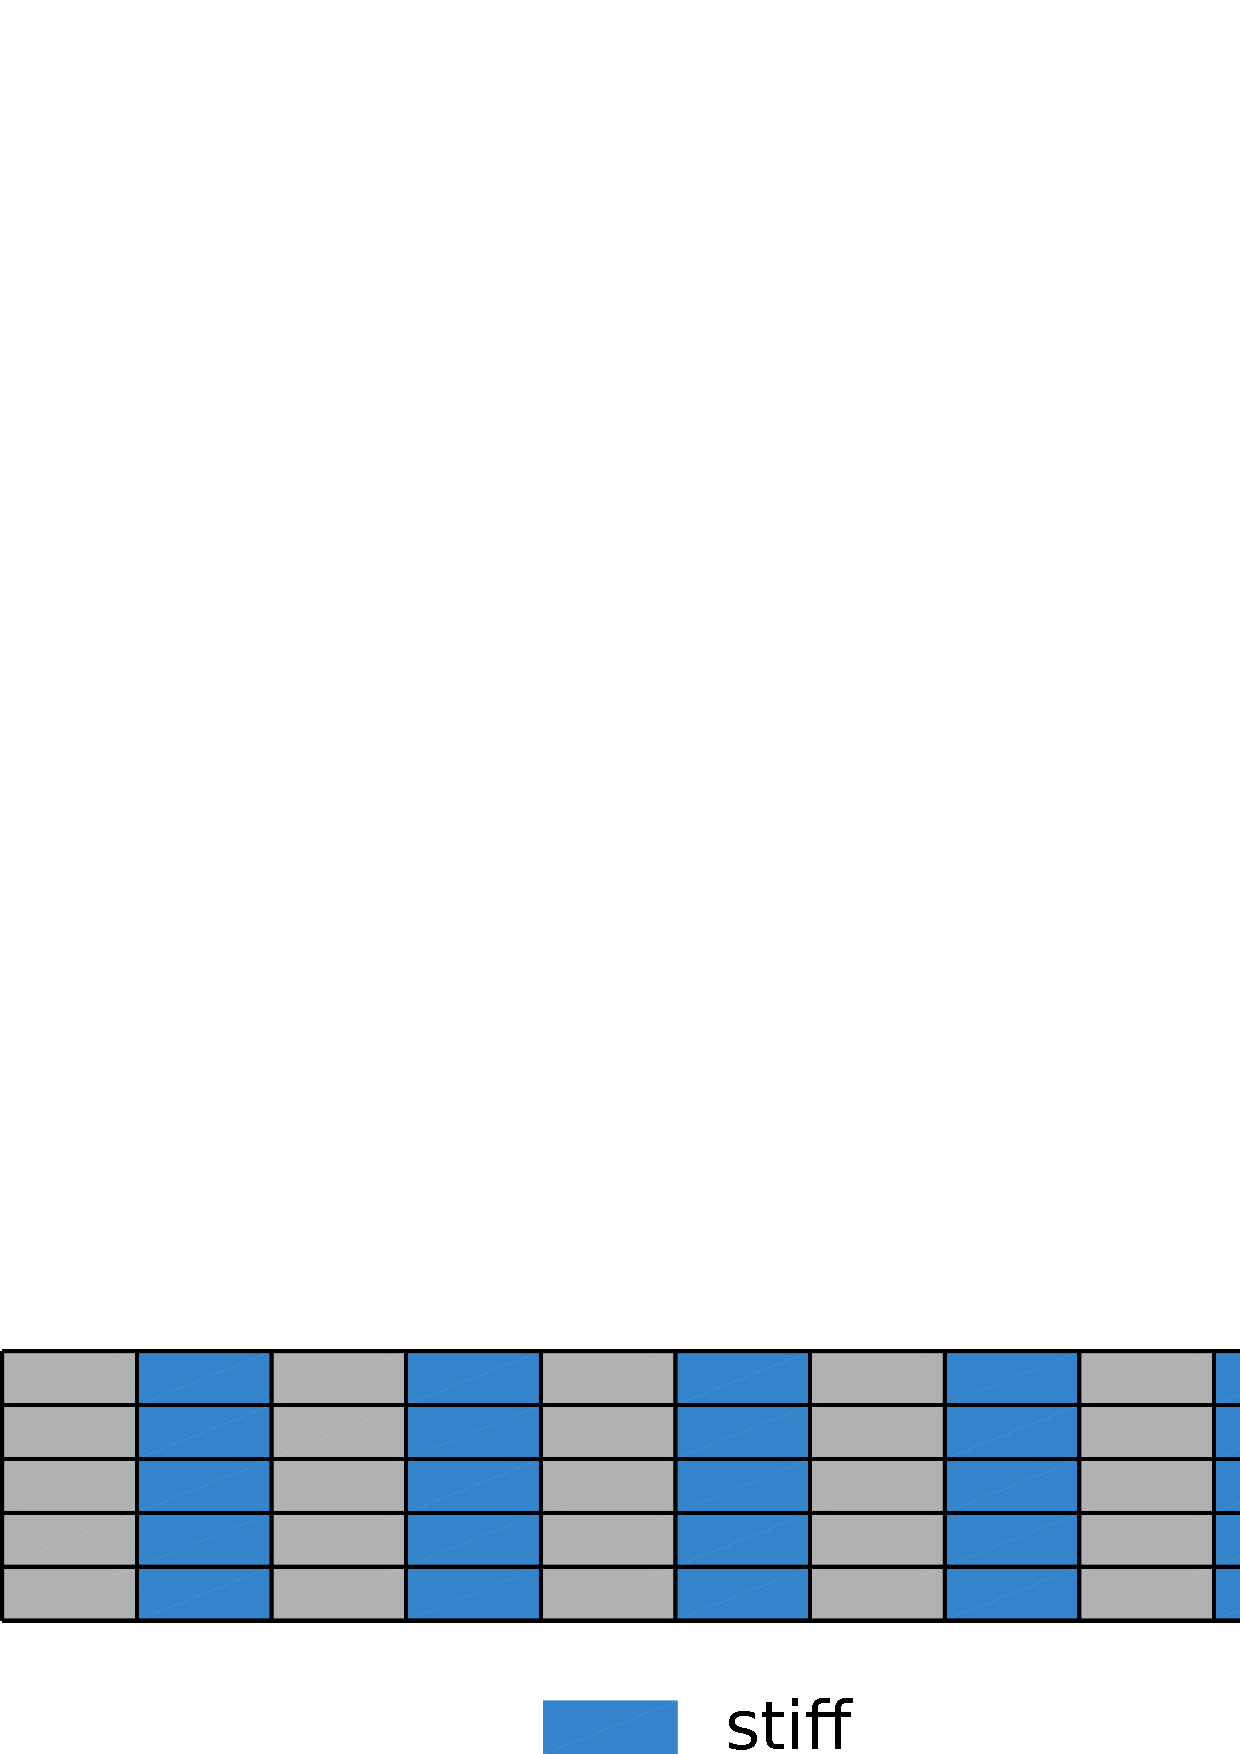
\includegraphics[width=.7\textwidth]{\studypath/2016-08-22_HeterogenityType/setup/materials_vertical.pdf}};
\node at (-5.5,\ydist) [anchor=north west, scale=0.7, white] {\contour{black}{iteration 2}}; 
    
\node[inner sep=0pt] (russell) at (0,2*\ydist)
    {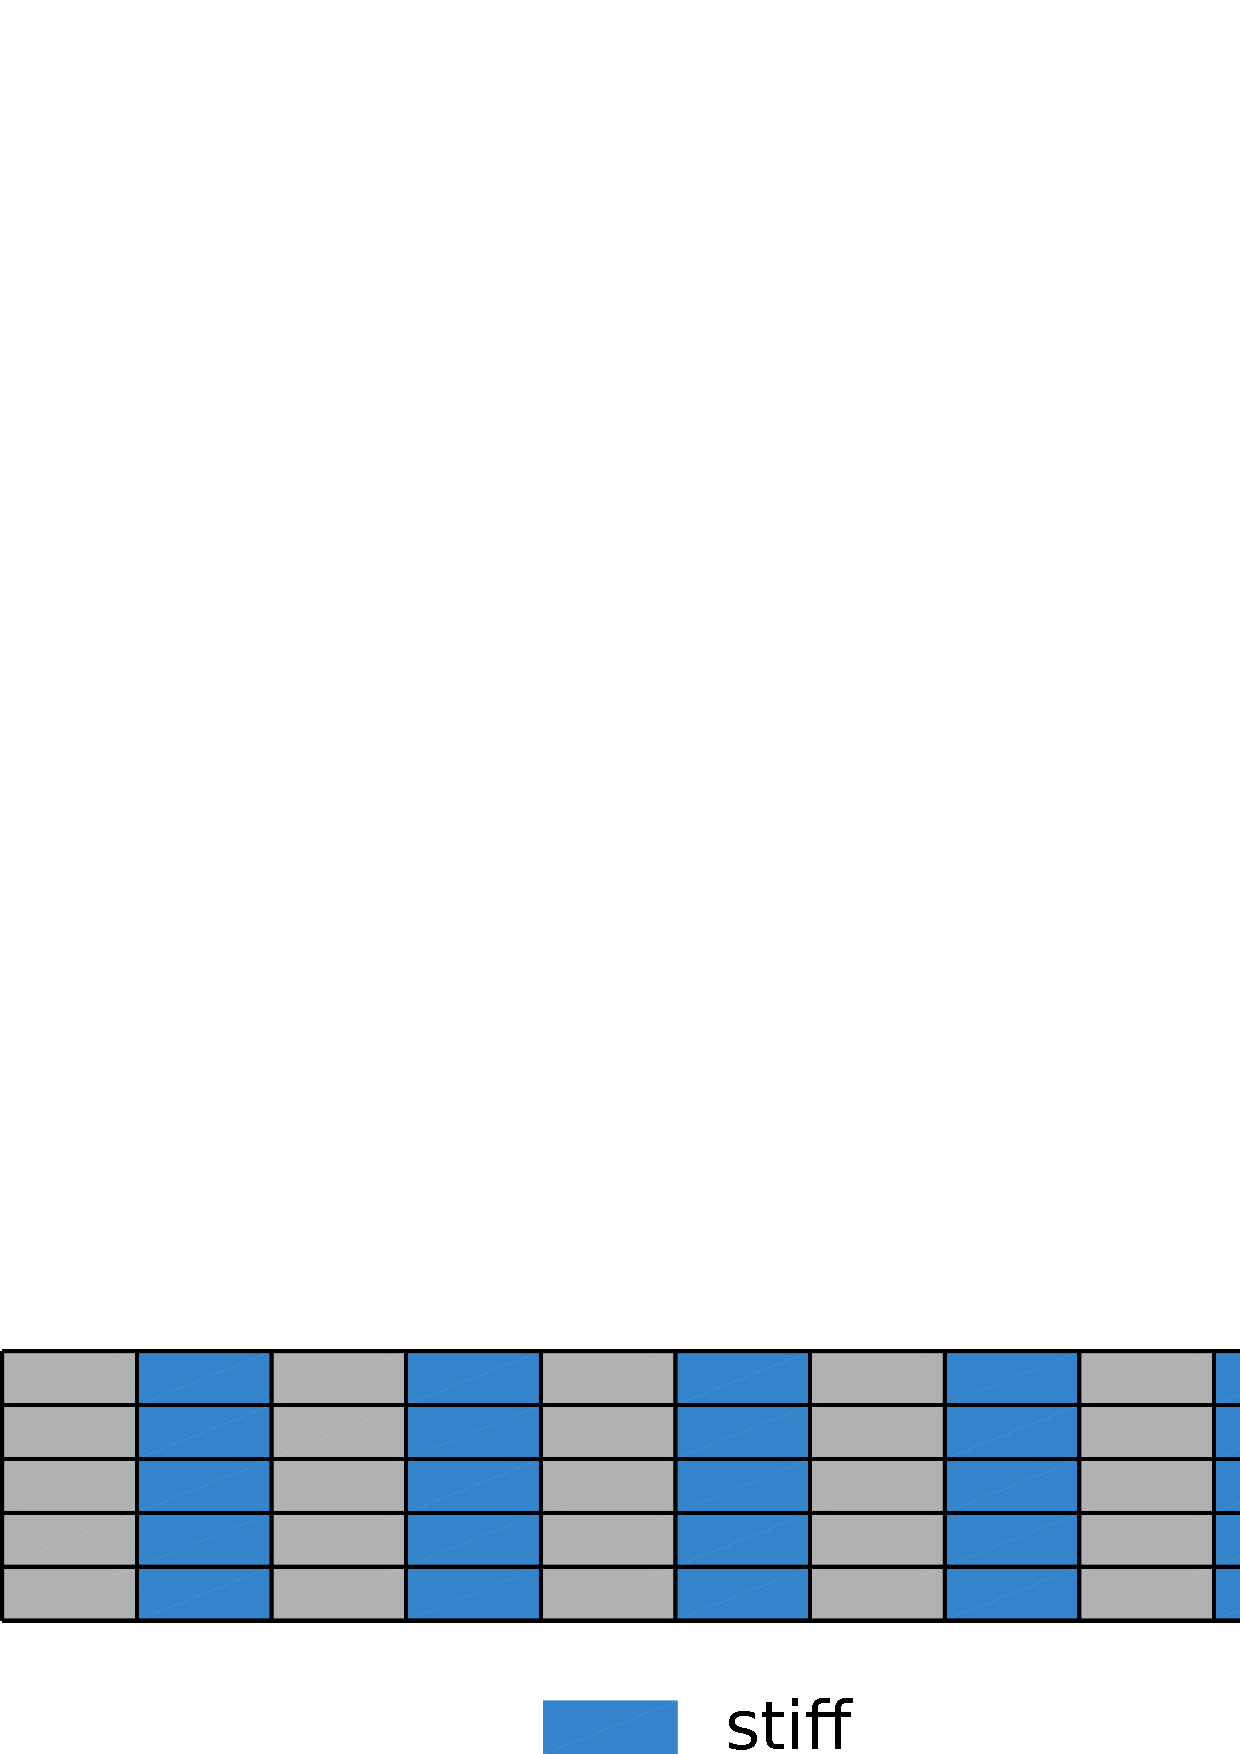
\includegraphics[width=.7\textwidth]{\studypath/2016-08-22_HeterogenityType/setup/materials_vertical.pdf}};
\node at (-5.5,2*\ydist) [anchor=north west, scale=0.7, white] {\contour{black}{iteration 3}}; 
    
\node[inner sep=0pt] (russell) at (0,3*\ydist)
    {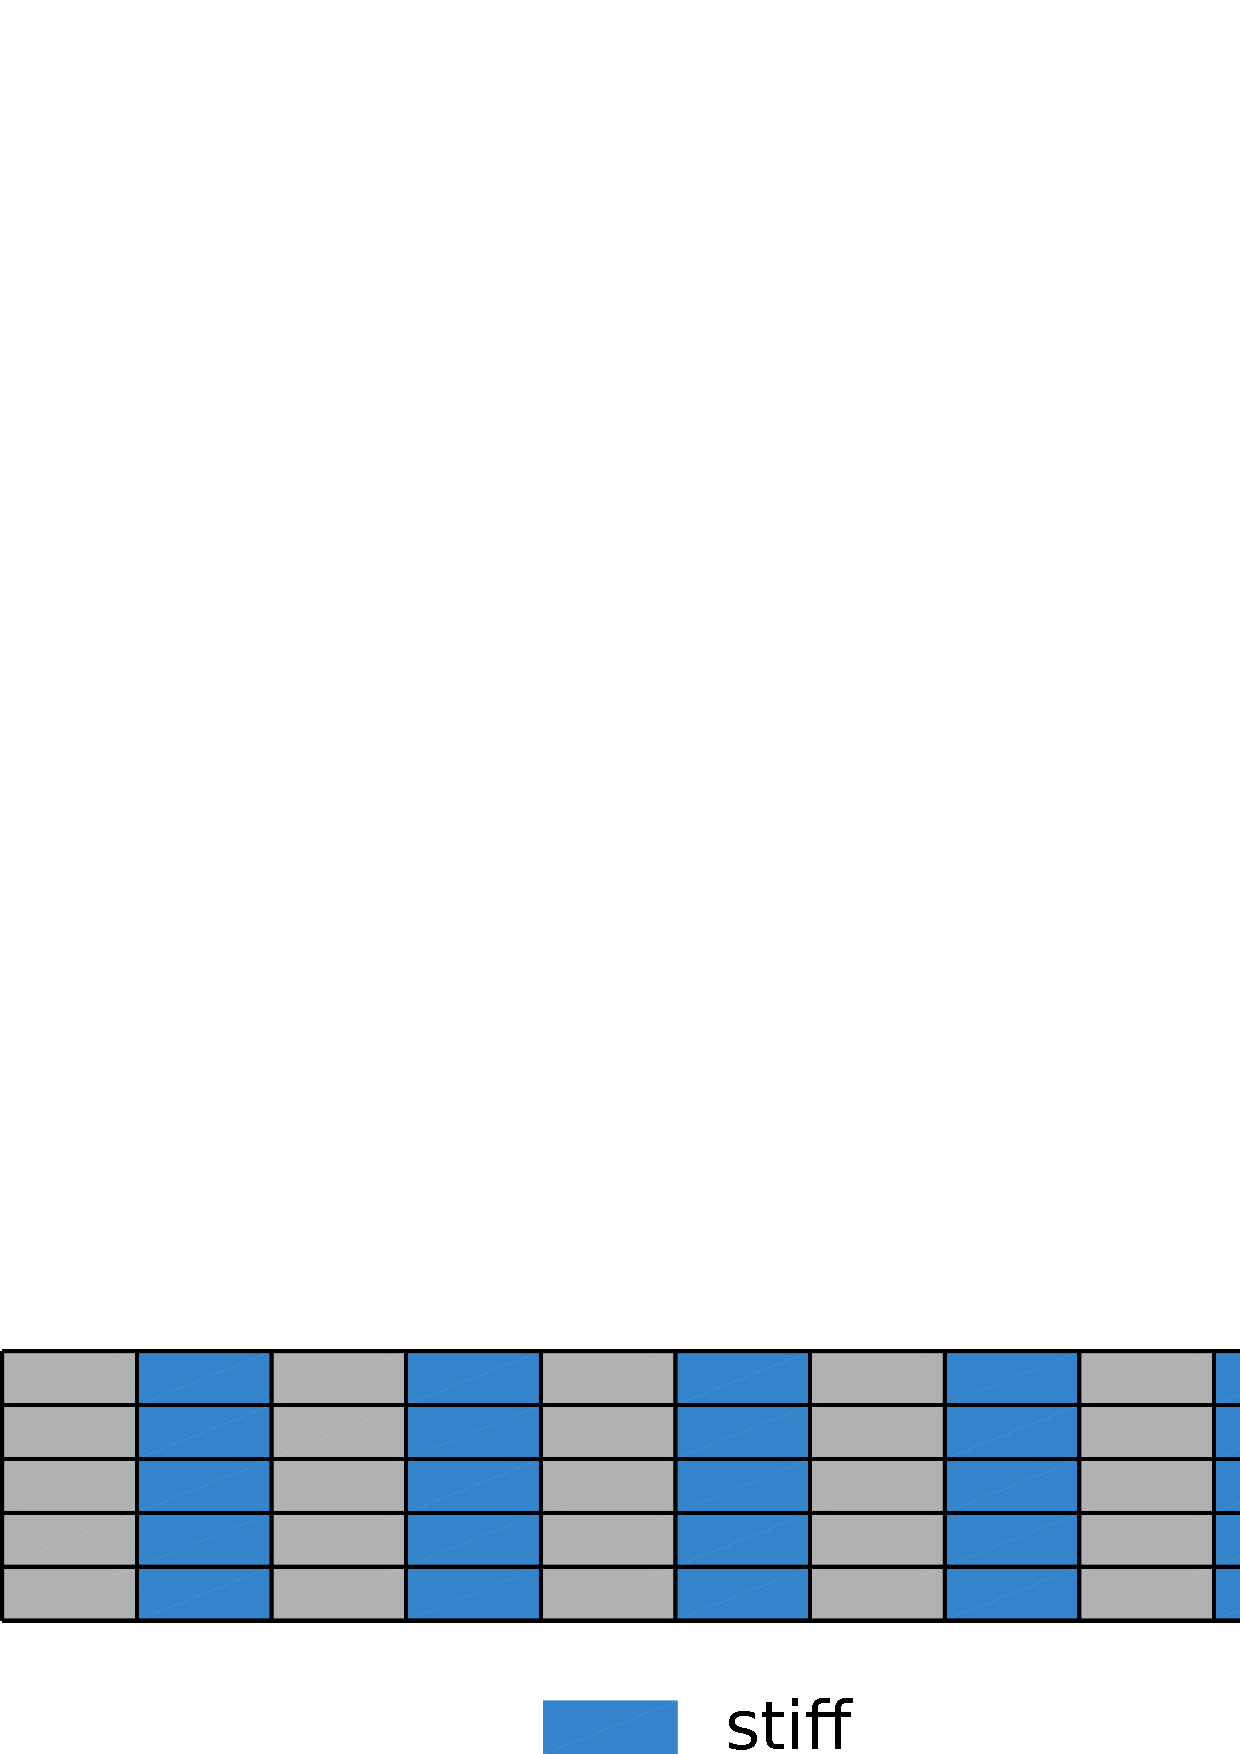
\includegraphics[width=.7\textwidth]{\studypath/2016-08-22_HeterogenityType/setup/materials_vertical.pdf}};
\node at (-5.5,3*\ydist) [anchor=north west, scale=0.7, white] {\contour{black}{converged~~}}; 
    
\end{tikzpicture}



\end{document}